\PassOptionsToPackage{table,xcdraw}{xcolor}
\documentclass[11pt]{article}
\usepackage{helvet}
%\bibliographystyle{plainat}
\usepackage{amsmath}
\usepackage{amssymb}
\usepackage{amsthm}
\usepackage{dsfont}
\usepackage[margin=1in]{geometry}
\usepackage{hyperref}
\usepackage{multirow}
\usepackage{color}
\usepackage{tikz}
\usepackage{graphicx}
\usepackage{setspace}
\usepackage{bigints}
\usepackage{bbm}
%\onehalfspacing
%\doublespacing
\usepackage{algorithm2e}
\usepackage{float}
\usepackage{lscape}
\usepackage{rotating}
\usepackage{longtable}
\usepackage{enumerate}
\usepackage{mdframed}
\usepackage{framed}
\usepackage{url}
\usepackage[table,xcdraw]{xcolor}
\usepackage{graphicx}
\usepackage{algorithm}
\usepackage{algpseudocode}  % Algorithm typesetting
\usepackage{indentfirst}
\usepackage{listings}
\usepackage{cite}
\usepackage[utf8]{inputenc}
\usepackage{tcolorbox}
\usepackage{booktabs}
\usepackage[normalem]{ulem}
\useunder{\uline}{\ul}{}

\newtcbox{\inlinecode}{on line, boxrule=0pt, boxsep=0pt, top=2pt, left=2pt, bottom=2pt, right=2pt, colback=gray!15, colframe=white, fontupper={\ttfamily}}

\newtheorem{lemma}{Lemma}
\newtheorem{theorem}{Theorem}
\newtheorem{proposition}{Proposition}
\newtheorem{definition}{Definition}
\newtheorem{assumption}{Assumption}
\hypersetup{
    colorlinks=true,
    linkcolor=black,
    filecolor=magenta,      
    urlcolor=blue,
    citecolor=black,
}


\newcommand{\indep}{\mathrel{\text{\scalebox{1.07}{$\perp\mkern-10mu\perp$}}}}
\DeclareMathOperator*{\argmin}{arg\,min}
\DeclareMathOperator*{\argmax}{arg\,max}
\newcommand{\bm}[1]{\mathbf{#1}}
\newcommand{\bs}[1]{\boldsymbol{#1}}
\newcommand{\E}{\mathbb{E}}
\newcommand{\V}{\mathbb{V}}
\newcommand{\I}{\mathbb{I}}
\newcommand{\com}[1]{&&\mbox{(#1)}}
\newcommand{\note}[1]{\noindent{\color{red} [\textbf{Note:} #1]}}
\NewDocumentCommand{\codeword}{v}{%
\texttt{\textcolor{blue}{#1}}%
}


\NewDocumentCommand{\setword}{v}{%
\texttt{\textcolor{black}{#1}}%
}


\newif\ifsoln
\solntrue

\usepackage{caption}
\newcommand*{\SHOWANSWERS}{}
\usepackage{enumitem}
%\usepackage[shortlabels]{enumitem}
%\lstset{language=C, keywordstyle = {\bfseries \color{blue}}}

\title{Airbnb Price Prediction Using Machine Learning}
\author{Linlin Li}
\date{November 16th\\ \href{https://www.kaggle.com/c/duke-cs671-fall20-airbnb-pricing-data}{Link}}

\begin{document}

\maketitle

\section{Background}
Airbnb is an online marketplace for vacation rentals that provides arrangements for lodging, primarily homestays, or tourism experiences. Homeowners can put their property online so that guests can pay to stay in them. The platform does not own any of the properties and does not host events. It acts as a broker and collects commissions from each booking. Although Airbnb and other websites may provide some general guidance, the price of each property is determined by its host. Appropriate prices are needed, because too high a price will result in a low booking rate, and too low a price will result in a loss of potential revenue. When determining the price, many factors should be considered, such as location, capacity, room type, etc. 

In this project, I am going to look at Airbnb listings in Buenos Aires and trying to provide some exploratory analysis around predicting listing prices. First, I will use Exploratory Data Analysis (EDA) to get to know the data. This will help me get an initial sense of which variables are associated with price, and which variables to include in the model. Using the important variables identified in EDA, I will try several classification models attempting to predict the price. Finally, I will evaluate the performance of the model.

\section{Exploratory Analysis}

To begin with the EDA, first I got a summary of the variables using \texttt{pandas\_profiling}
\cite{pandasprofiling2019} . For the full details, feel free to check the Appendix \ref{code}. There are 9681 listings in the training set, which contains 24 features. The following are my findings:
\begin{itemize}
    \item There are no missing values in the training set.
    \item \inlinecode{is\_business\_travel\_ready} is the same for all observations, so it cannot provide any information for the price. I choose to remove it. 
    \item There are many binary variables. I will convert them into dummy variables after EDA.
    \item \inlinecode{host\_since} is a datetime column and should be converted into metric that measures the number of days the host has been on Airbnb. I used November 5th, 2020 to calculate this metric and named it \inlinecode{host\_days\_active}. Similarly, \inlinecode{last\_review} is converted to \inlinecode{time\_since\_last\_review}.
    \item \inlinecode{require\_guest\_phone\_verification} and \inlinecode{require\_guest\_profile\_picture} are highly correlated.
    \item \inlinecode{number\_of\_reviews} and \inlinecode{reviews\_per\_month} are highly correlated. This is reasonable because the latter is the "average value" of the former.
    \item \inlinecode{bedrooms}, \inlinecode{beds} and \inlinecode{bathrooms} are highly correlated. The number of beds has traditionally been a more high priority search parameter on Airbnb, as it is more relevant for the number of people accommodated than the number of bedrooms (and is still the second highest priority parameter when searching on the site. In addition, \inlinecode{guests\_included} is correlated with these three variables.
\end{itemize}

\subsection{Investigating Binary Variables}
Next, I noted that a large amount of the variables are binary. I investigated the association with price via stacked bar plots. 
\begin{figure}[h]
    \caption{Stacked bar plots between price and some binary variables}
    \label{binary}
    \centering
    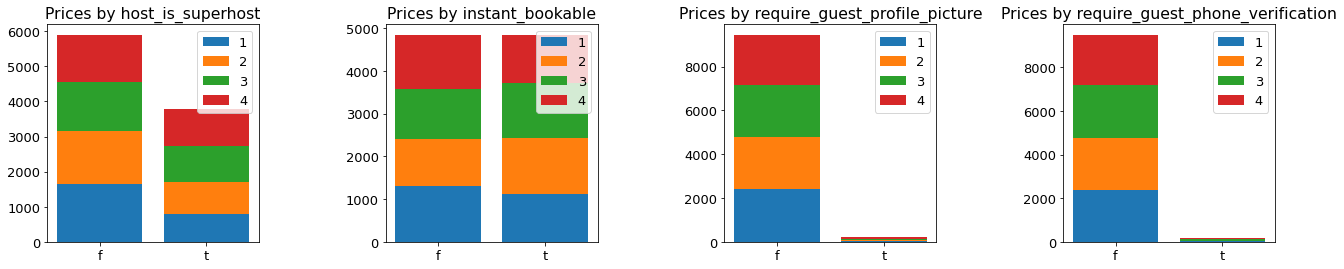
\includegraphics[width=1.15\textwidth]{../img/binary.png}
\end{figure}

Figure \ref{binary} provide a great visualization on how a given binary variable is associated with changes in price. I saw the following findings from the graph:
\begin{itemize}
    \item \inlinecode{host\_is\_superhost} seems to be a potential predictor because the distribution of price is different between the two categories of \inlinecode{host\_is\_superhost}.
    \item The difference in the distribution of price in the two categories of \inlinecode{instant\_bookable} seems to be trivial, maybe \inlinecode{instant\_bookable} cannot provide much information about price. I will drop it after EDA. 
    \item The distribution of price for \inlinecode{require\_guest\_phone\_verification} and \newline \inlinecode{require\_guest\_profile\_picture} are very similar. Since these two variables are highly correlated, we can simply drop one of them. I choose to drop \inlinecode{require\_guest\_profile\_picture} after EDA because I think phone verification is more strict.
\end{itemize}

\subsection{Investigating Categorical Variables}

Several variables have multiple categories (\inlinecode{room\_type}, \inlinecode{bed\_type} and \inlinecode{cancellation\_policy}). I can also visualize these with stacked bar plots, there will just be more bars than a binary variable. 

\begin{figure}[H]
    \caption{Stacked bar plots between price and some categorical variables}
    \label{categorical}
    \centering
    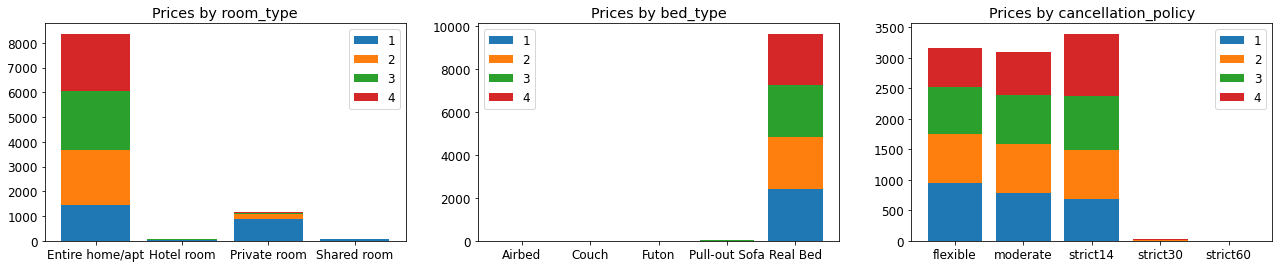
\includegraphics[width=1.15\textwidth]{../img/categorical.png}
\end{figure}

Figure \ref{categorical} provide a great visualization on how a given categorical variable is associated with changes in price. 
\begin{itemize}
    \item Several of the categories for variables have very small sample sizes (\inlinecode{bed\_type} and \inlinecode{cancellation\_policy}). 
    \begin{itemize}
        \item[--]  For \inlinecode{cancellation\_policy}, `super\_strict\_30' and `super\_strict\_60' only appear in 26 and 3 listings respectively, which are very small in the training set. Since the super strict options are only available to long-term Airbnb hosts and is invitation only, it is clear that the super strict options are stricter than `strict\_14\_with\_grace\_period'. As the number of `super strict' is too small, I will combine it with `strict\_14\_with\_grace\_period' after EDA.
        \item[--] Similarly, for \inlinecode{bed\_type}, I will combine `Couch' and `Airbed' into `other' after EDA. 
    \end{itemize}
    \item It would make sense that \inlinecode{room\_type} could be an important factor; perhaps certain rooms types are more private and therefore more expensive.
    \item The association between \inlinecode{cancellation\_policy} and price does not seem so close, which is a bit counterintuitive, because customers tend to pay higher prices when choosing a more flexible policy.
    \item For \inlinecode{neighbourhood}, I also combine those classes with particularly small sample sizes ($< 7$) with `other'.
\end{itemize} 

\subsection{Investigating Numerical Variables}
Finally, certain variables are continuous in nature. We can investigate the relationship with price via boxplots. Figure \ref{numerical} provide a great visualization on how a given numerical variable is associated with changes in price. 


\begin{itemize}
    \item \inlinecode{minimum\_nights} and \inlinecode{maximum\_nights} seem to provide very little information about price. 
    \item It seems that \inlinecode{bathrooms}, \inlinecode{bedrooms}, \inlinecode{cleaning\_fee}, \inlinecode{guests\_included}, \inlinecode{availability\_365}, \inlinecode{cleaning\_fee}, and \inlinecode{calculated\_host\_listings\_count} are influencing factors. 
\end{itemize}

\begin{figure}[H]
    \caption{Boxplots between price and some numerical variables}
    \label{numerical}
    \centering
    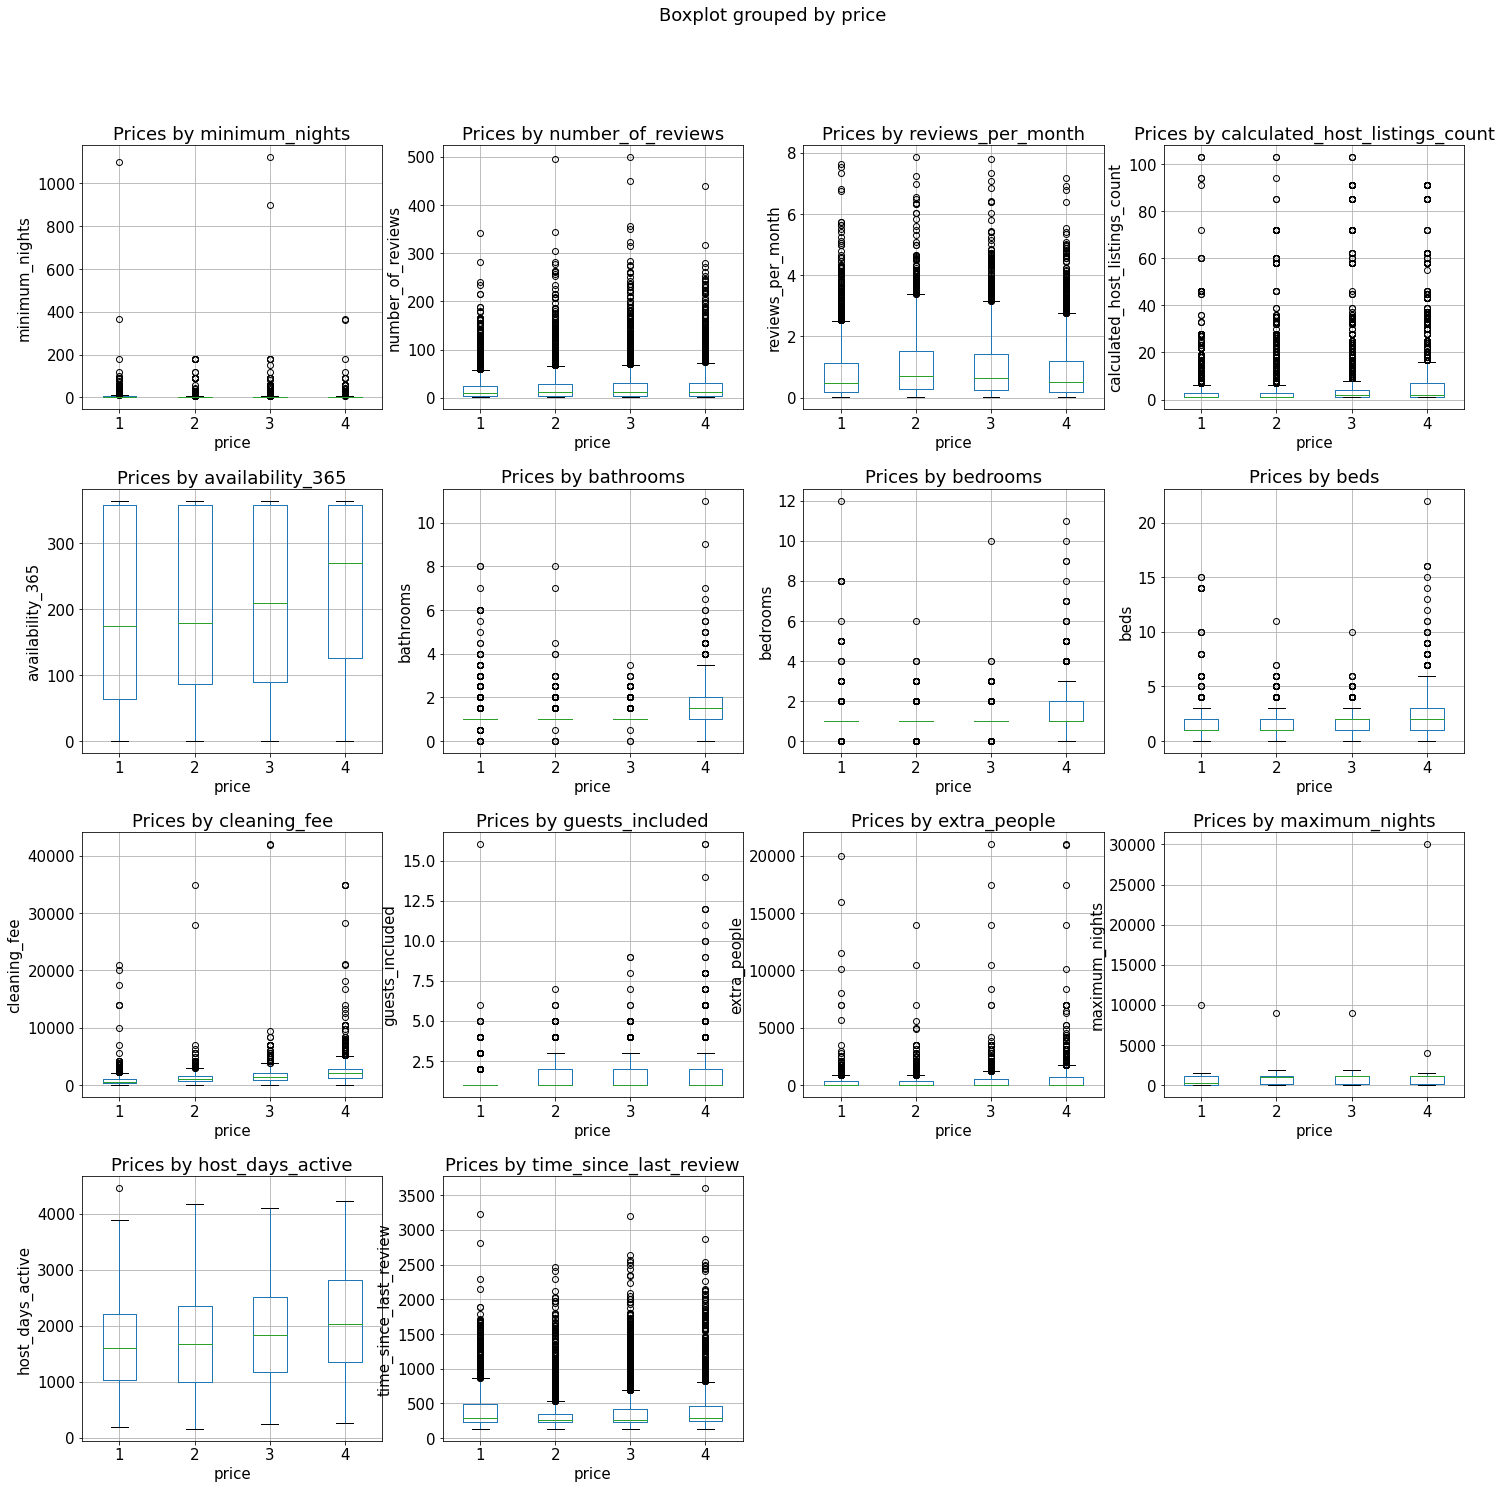
\includegraphics[width=1.15\textwidth]{../img/numerical.png}
\end{figure}


\section{Data Splits}

After performing EDA, I divided the training set into two parts: about 70\% of the training set (6776 records) was used for training, and the remaining 30\% of the training set (2905 records) was reserved for testing the out-of-sample performance. 

In the hyperparameter selection part, I used 10-fold cross-validation on my training set (6776 records) and divided it into 10 folds. Each time I set aside 1 fold for testing and trained the classifier on the other 9 folds and evaluated the categorization accuracy on the 1 fold. After adjusting the hyperparameters, I computed the out-of-sample accuracy of each of my models on my test set (2905 records).

\section{Models}

After cleaning and dropping columns, the available features in the model are:
\begin{itemize}
    \item Room type
    \item Minimum and maximum nights stay
    \item Total number of reviews
    \item Average number of reviews left by guest each month
    \item How many listings the host is responsible for in total 
    \item Number of days available to book in the next 365 days
    \item Whether or not a host is a superhost, has their identity verified (e.g. by verifying a phone number)
    \item The number of bathrooms, bedrooms, and beds
    \item Type of bed
    \item Cleaning fee and extra person fee
    \item The number of guests included in the booking fee
    \item The type of cancellation policy
    \item How many days the host has been listing on Airbnb
    \item Amount of time since the most recent reviews
    \item Neighborhood
\end{itemize}

The continuous variables were standardized using \texttt{scikit-learn}’s \texttt{StandardScaler()}. Categorical features were encoded into indicator variables using \texttt{pandas.get\_dummies()}. 

In order to have a basic sense of which algorithms to go. I first tried many baseline classification models using \texttt{compare\_models()} from \texttt{PyCaret}\cite{PyCaret}, which is an end-to-end machine learning and model management tool that automates machine learning workflows and accelerate the experiment cycle exponentially. Due to limited time and computating resources, I used the default setting of \texttt{compare\_models()}, where some models that require a long running time are prevented for comparison. Table \ref{table:baseline} displays the results of models with default hyperparameters using 10-fold cross-validation on my training set (6776 records).

Random forest and some boosting algorithms seem to perform better than others. Thanks to the high-quality libraries available online, these algorithms are easy to train and use for prediction. In the next section, I will try these algorithms, and tune their hyperparameters. 

\begin{table}[h]
\begin{center}
    \begin{tabular}{llllllll}
    \toprule
    \textbf{} &
      \textbf{Model} &
      \textbf{Accuracy} &
      \textbf{AUC} &
      \textbf{Recall} &
      \textbf{Prec.} &
      \textbf{F1} &
      \textbf{TT (Sec)} \\
\midrule
    \textbf{rf} &
{Random Forest Classifier} &
\textcolor{red}{0.5403} & \textcolor{red}{0.7933} & \textcolor{red}{0.5420} & \textcolor{red}{0.5485} & \textcolor{red}{0.5432} & {0.2170} \\
\textbf{lightgbm} &
  Light Gradient Boosting Machine &
       {0.5331} & {0.7919} & {0.5346} & {0.5410} & {0.5359} & 0.1160 \\
{\textbf{catboost}} &
  {CatBoost Classifier} & {0.5319} & {0.7894} & {0.5337} & {0.5366} & {0.5334} & {3.9600} \\
{\textbf{xgboost}} &
  {Extreme Gradient Boosting} &
  {0.5298} & {0.7888} & {0.5310} & {0.5381} & {0.5328} & {1.4750} \\
{\textbf{gbc}} &
  {Gradient Boosting Classifier} & 
  {0.5283} & {0.7844} & {0.5301} & {0.5396} & {0.5323} & {0.6360} \\
{\textbf{et}} &
  {Extra Trees Classifier} &
  {0.5252} & {0.7753} & {0.5270} & {0.5309} & {0.5271} & {0.1610} \\
{\textbf{ada}} &
  {Ada Boost Classifier} &
  {0.4993} & {0.7371} & {0.5012} & {0.5045} & {0.5009} & {0.0630} \\
{\textbf{lr}} &
  {Logistic Regression} &
  {0.4907} & {0.7564} & {0.4929} & {0.5011} & {0.4942} & {0.1970} \\
{\textbf{lda}} &
  {Linear Discriminant Analysis} &
  {0.4824} & {0.7474} & {0.4836} & {0.5232} & {0.4921} & {0.0200} \\
{\textbf{ridge}} &
  {Ridge Classifier} &
  {0.4777} & {0.0000} & {0.4805} & {0.4832} & {0.4780} & {0.0750} \\
{\textbf{knn}} &
  {K Neighbors Classifier} &
  {0.4604} & {0.7026} & {0.4616} & {0.4720} & {0.4618} & {0.2630} \\
{\textbf{dt}} &
  {Decision Tree Classifier} &
  {0.4451} & {0.6294} & {0.4463} & {0.4476} & {0.4452} & {0.0840} \\
{\textbf{svm}} &
  {SVM - Linear Kernel} &
  {0.4418} & {0.0000} & {0.4438} & {0.4474} & {0.4184} & {0.1200} \\
  \bottomrule
\end{tabular}
\end{center}
\caption{ Baseline classification models. Results are based on 10-fold cross-validation on my training set (6776 records). Table is sorted by accuracy. Certain models are prevented for comparison because of their longer run-time.}
\label{table:baseline}
\end{table}


\section{Training}

\subsection{ Random Forest Classifier}
In the random forest classifier, each tree in the ensemble is built from a sample drawn with replacement (i.e., a bootstrap sample) from the training set\cite{ho1998random}. When splitting each node during the construction of a tree, the best split is found from a random subset of variables\cite{ho1998random}. The purpose of these two sources of randomness is to decrease the variance of the forest estimator\cite{ho1998random}. Random forests achieve a reduced variance by combining diverse trees, sometimes at the cost of a slight increase in bias\cite{ho1998random}. The \texttt{scikit-learn} implementation combines classifiers by averaging their probabilistic prediction, instead of letting each classifier vote for a single class\cite{scikit-learn}.

It took about 6.58 seconds (wall time) to train a random forest classifier on the whole training set (9681 records).

\subsection{ Gradient Boosting Classifier }

In boosting, the individual models are not built on completely random subsets of data and features but sequentially by putting more weight on instances with wrong predictions and high errors\cite{friedman2002stochastic}. In each round of training, the weak learner is built and its predictions are compared to the correct outcome that we expect\cite{friedman2002stochastic}. The distance between prediction and truth represents the error rate of our model, which can be used to calculate the gradient\cite{friedman2002stochastic}. The gradient can be used to find the direction in which to change the model parameters in order to (maximally) reduce the error in the next round of training by “descending the gradient”\cite{friedman2002stochastic}.

In Gradient Boosting, we are combining the predictions of multiple models, we are not optimizing the model parameters directly but the boosted model predictions\cite{friedman2002stochastic}. 

It took about 26.6 seconds (wall time) to train a gradient boosting classifier on the whole training set (9681 records).

\subsection{ XGBoost Classifier}

XGBoost, also called Extreme Gradient Boosting, is a specific implementation of the Gradient Boosting method which uses more accurate approximations to find the best tree model\cite{chen2015xgboost}. While regular gradient boosting uses the loss function of the base model (e.g. decision tree) as a proxy for minimizing the error of the overall model, XGBoost uses the second-order derivative as an approximation, which tends to provide more information about the gradients\cite{chen2015xgboost}.

It took about 11.3 seconds (wall time) to train a XGBoost classifier on the whole training set (9681 records).

\section{Hyperparameter Selection}

\subsection{ Random Forest Classifier}
In the random forest model, I tried to tune ``criterion'' and ``n\_estimators''. I used grid search to get the accuracy using 10-fold cross-validation on my training set (6776 records). Figure \ref{cv_rf} shows the cross-validation accuracy on my training set and these two hyperparameters. 

\begin{figure}[H]
  \caption{Cross-validation accuracy using Random Forest Classifier on my training set (6776 records).}
  \label{cv_rf}
  \centering
  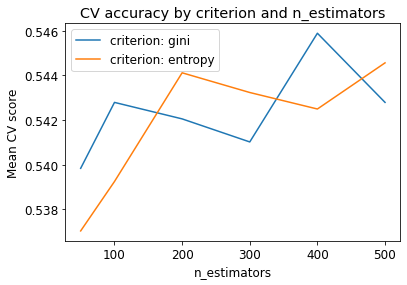
\includegraphics[width=0.65\textwidth]{../img/cv_rf.png}
\end{figure}

As can be seen in Figure \ref{cv_rf}, the best combinations of these two hyperparameters is ``criterion = `gini' '' and ``n\_estimators=400''.

\subsection{ Gradient Boosting Classifier }
In the gradient boosting model, I tried to tune ``learning\_rate'' and ``n\_estimators''. I used grid search to get the accuracy using 10-fold cross-validation on my training set (6776 records). Figure \ref{cv_gbc} shows the cross-validation accuracy on my training set and these two hyperparameters. 

\begin{figure}[H]
  \caption{Cross-validation accuracy using Gradient Boosting Classifier on my training set (6776 records).}
  \label{cv_gbc}
  \centering
  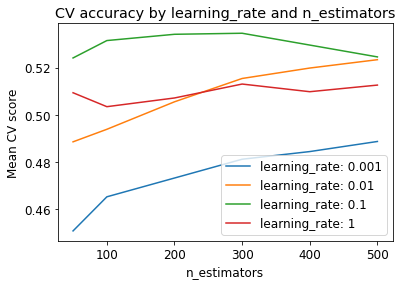
\includegraphics[width=0.65\textwidth]{../img/cv_gbc.png}
\end{figure}

As can be seen in Figure \ref{cv_gbc}, the best combinations of these two hyperparameters is ``learning\_rate = 0.1 '' and ``n\_estimators=300''.

\subsection{ XGBoost Classifier}
In the XGBoost model, I tried to tune ``learning\_rate'' and ``n\_estimators''. However, due to limited computing resources, I cannot directly use grid search to get the results using 10-fold cross-validation on my training set (6776 records). In this case, I tried to manually calculated the 10-fold cross-validation accuracy for each combinations of hyperparameters. Figure \ref{cv_xgbc} shows the cross-validation accuracy on my training set and these two hyperparameters. 

\begin{figure}[H]
  \caption{Cross-validation accuracy using XGBoost Classifier on my training set (6776 records).}
  \label{cv_xgbc}
  \centering
  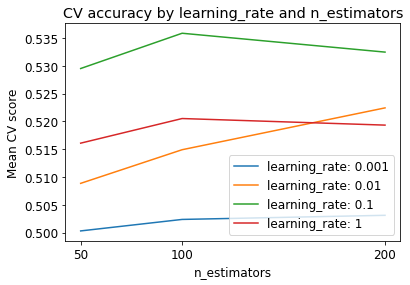
\includegraphics[width=0.65\textwidth]{../img/cv_xgbc.png}
\end{figure}

As can be seen in Figure \ref{cv_xgbc}, the best combinations of these two hyperparameters is ``learning\_rate = 0.1 '' and ``n\_estimators=100''.

\section{ Stacked Models}
One possible way to improve the predictive accuracy is to combine different models. Stacking (sometimes called ``stacked generalization'') involves training a new learning algorithm to combine the predictions of several base learners\cite{boehmke2019hands}. First, the base learners are trained using the available training data, then a combiner or meta algorithm, called the super learner, is trained to make a final prediction based on the predictions of the base learners\cite{boehmke2019hands}. Figure \ref{stacked} shows the struc
Such stacked ensemble often outperforms any of the individual base learners (e.g., a single random forest) and has been shown to represent an asymptotically optimal system for learning \cite{van2007super}.

I tried to stack the predictions from the top 7 classifiers in Table \ref{table:baseline} up to get a final prediction using a linear model as the combiner. All of these 7 classifiers form the base layer of the stack, and their predictions are used as input to the meta model. It is very convenient to do this by \texttt{stack\_models()} in \texttt{PyCaret}. Similarly, the output of this function is the result of the stacked models using 10-fold cross-validation.

\begin{figure}[h]
  \caption{Stacked Models}
  \label{stacked}
  \centering
  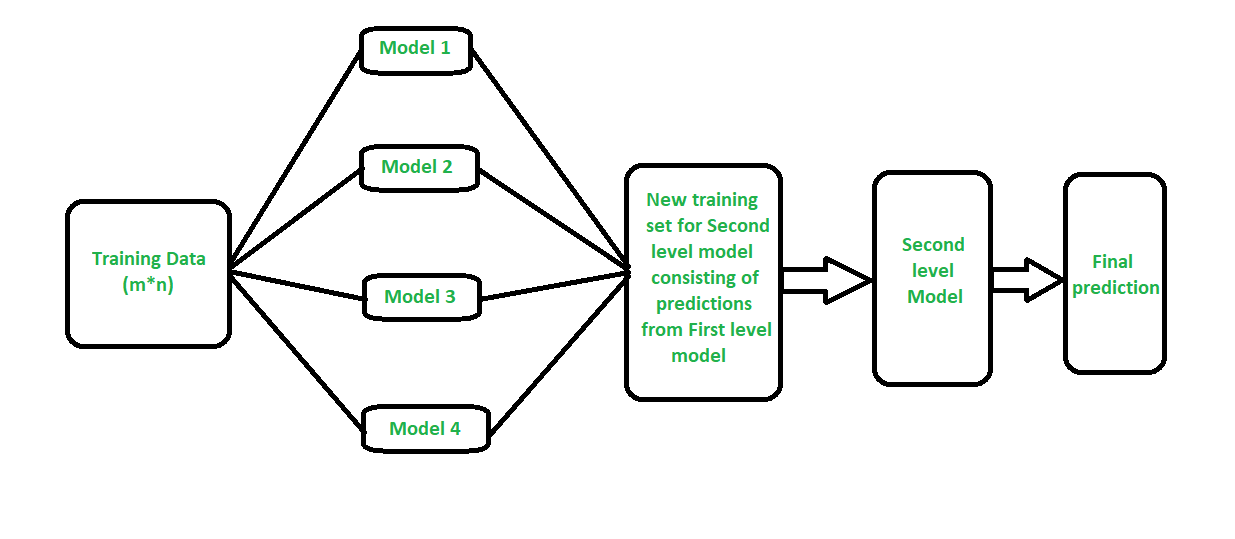
\includegraphics[width=\textwidth]{../img/stacking.png}
\end{figure}

\section{Errors and Mistakes}

This competition is not that easy as it seems to be. For me, feature selection is the hardest part. In the original dataset, there are 24 features (except the response), including DateTime features, categorical features, and numeric features. Additionally, some features are highly correlated, which increases the demand for feature selection and increases the difficulty for modeling. If I delete too many features, I will lose too much information about prices; if I keep too many unnecessary features, the predictive accuracy may not be satisfactory.

\section{Predictive Accuracy}

My Kaggle username is Linlin Li. Table \ref{compare} displays the performance of my models. 

\begin{table}[h]
    \centering
    \begin{tabular}{lllll}
    \toprule
    & Models & CV Accuracy & Out-of-sample Accuracy & Test Accuracy$^*$\\
    \midrule
    \textbf{rf}  & Random Forest Classifier &  0.5494  &  0.5491  &  0.5643   \\  
    \textbf{gbc} & Gradient Boosting Classifier &  0.5331  &  0.547  &  0.5402   \\  
    \textbf{xgboost} & Extreme Gradient Boosting &  0.5342  &  0.5497  &  0.545   \\  
    \textbf{stacked5} & Stacked model of 5 base learners &  0.5502  &  0.559  &   0.5619  \\  
    \textbf{stacked7} & Stacked model of 7 base learners  &  0.55  &  0.5608  &   \textcolor{red}{0.5788}  \\  
    \textbf{stacked10} & Stacked model of 10 base learners  &  0.5561  &  0.5597  &   0.5691  \\  
    \bottomrule    
    \end{tabular}
    \caption{Categorization accuracy of models on the training set and the test set. Out-of-sample accuracy was obtained on my test set (2905 records). Note that test accuracy was obtained from Kaggle (based on 30\% of test set). For each model, I've submitted several versions to Kaggle and the results here in test accuracy are the best among each model.}
    \label{compare}
\end{table}

From Table \ref{compare}, ``stacked7'' is probably my best model, which performs slightly better than other models on both my test set and the test set on Kaggle. We can visualize its performance on the out-of-sample data (2905 records) in Figure \ref{confusionmatrix} and \ref{auc}. 

From the confusion matrix (Figure \ref{confusionmatrix}) of the model, we can see that the overall performance of the model seems to be good. And it performs better on class 1 and 4 than on class 2 and 3. 

In a multi-class model, we can plot $K$ number of ROC Curves for $K$ number classes using One vs ALL methodology. For Example, if you have three classes named X, Y, and Z, you will have one ROC for X classified against Y and Z, another ROC for Y classified against X and Z, and the third one of Z classified against Y and X. As shown in Figure \ref{auc}, AUC for each class is at least 0.73, which is much greater than 0.5, which means that there is at least 73\% chance that the model will be able to distinguish each class from the other classes.

\begin{figure}[h]
  \caption{Confusion matrix of the stacked model of 7 base learners on my test data (2905 records).}
  \label{confusionmatrix}
  \centering
  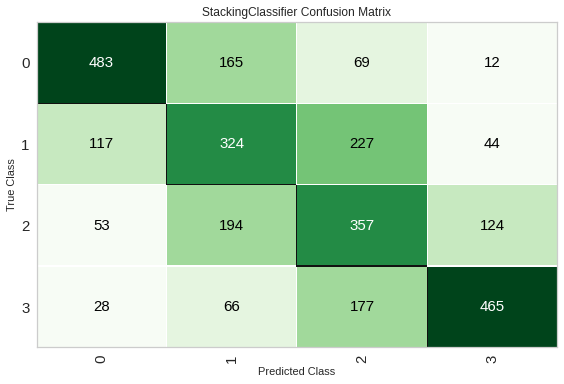
\includegraphics[width=0.7\textwidth]{../img/confusionmatrix.png}
\end{figure}

\begin{figure}[H]
  \caption{AUC curve for the stacked model of 7 base learners on my test data (2905 records).}
  \label{auc}
  \centering
  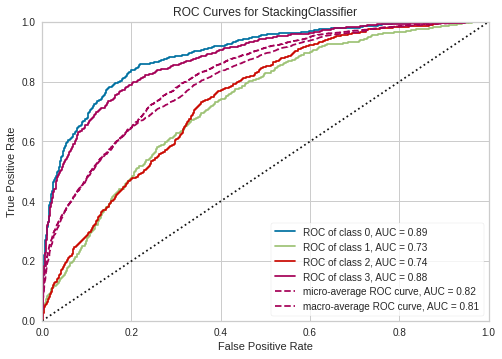
\includegraphics[width=0.7\textwidth]{../img/auc.png}
\end{figure}


\bibliographystyle{unsrt}
\bibliography{lit}


\end{document}